\documentclass[12pt]{article}

% fonts

\usepackage[scaled=0.92]{helvet}   % set Helvetica as the sans-serif font
\renewcommand{\rmdefault}{ptm}     % set Times as the default text font

\usepackage[T1]{fontenc}
\usepackage{amsmath}
\usepackage{amsfonts}

% page numbers
\usepackage{fancyhdr}
\fancypagestyle{newstyle}{
\fancyhf{} % clear all header and footer fields
\fancyfoot[R]{\vspace{0.1in} \small \thepage}
\renewcommand{\headrulewidth}{0pt}
\renewcommand{\footrulewidth}{0pt}}
\pagestyle{newstyle}

% geometry of the page
\usepackage[top=1in,
            bottom=1in,
            left=1in,
            right=1in]{geometry}

% paragraph spacing
\setlength{\parindent}{0pt}
\setlength{\parskip}{2ex plus 0.4ex minus 0.2ex}

% useful packages
\usepackage{natbib}
\usepackage{epsfig}
\usepackage{url}
\usepackage{bm}

%%%%%%%%%%%%%%%%%%%%%%%%%%%%%%%%%%% David's Additions %%%%%%%%%%%%%%%%%%%%%%%%%%

%% standard packages and arguments should be modified as needed
\usepackage{amssymb}
\usepackage{amsthm}
\usepackage[colorlinks=true,bookmarks=false,citecolor=blue,urlcolor=blue]{hyperref} %pdflatex
%\usepackage[breaklinks,colorlinks=true,bookmarks=false,citecolor=blue,urlcolor=blue]{hyperref} %latex w/dvipdf

\usepackage[english]{babel}
\newtheorem{theorem}{Theorem}
\newtheorem{corollary}{Corollary}
\newtheorem{lemma}[theorem]{Lemma}
\newtheorem{conjecture}{Conjecture}
\newtheorem{definition}{Definition}
\newtheorem{workdefinition}{Working Definition}
\newtheorem{problem}{Problem}
\newtheorem{example}{Example}
\newtheorem{remark}{Remark}

% \usepackage{color}
\usepackage[dvipsnames]{xcolor}
\newcommand\dashto{\mathrel{
  -\mkern-6mu{\to}\mkern-20mu{\color{white}\bullet}\mkern12mu
}}

\newcommand\indep{\perp \!\!\! \perp}

\usepackage{graphicx,centernot}
\newcommand{\CI}{\mathrel{\perp\mspace{-10mu}\perp}}
\newcommand{\nCI}{\centernot{\CI}}

% Usage
% $a \CI c \mid b$ and $a \nCI c \mid b$

\newcommand\R{\mathbb{R}}

\usepackage{caption}
\usepackage{subcaption}

\usepackage{dot2texi}

\usepackage{tikz}
% \usetikzlibrary{shapes,arrows}
\usetikzlibrary {graphs}

\begin{document}

\large \textbf{stable-Lipchitz SCMs: D-separation and Cyclic Causality} \\
% Reading: Title (Author, Year) \\
David Reber (dpr2127) \\
\today

\vspace{0.1in}

\normalsize

% Write here.



% \title{stable-Lipchitz SCMs: D-separation and Cyclic Causality}

% \author{David Reber}
% \address{Columbia University}
% \email{david.reber@columbia.edu}
%%Uncomment the following line to override copyright year from the default current year.
% \copyrightyear{2022}


\begin{abstract}
Despite being the natural modeling choice for phenomena involving feedback, cyclic causality has seen limited use because many of the convienent guarentees of acylic SCMs fail to hold for general cyclic SCMs. One well-known hurdle to this modeling option is that d-separation fails to hold for general cyclic SCMs.

In this report, we present research about the validity of d-separation (aka. the dGMP: directed global Markov property) for cyclic SCMs. Specifically, we propose the class of stable-Lipschitz SCMs, which generalize acyclic SCMs and are contained by simple SCMs. Stable-Lipschitz SCMs behave like linear SCMs asyptotically, and indeed, are proven to satsify the dGMP (currently with some additional constraints).
These results are verified numerically, and the validity of the backdoor adjustment criterion is proven as well. We further show that stable-Lipschitz SCMs are closed under interventions, and that the interventional distributions of simple SCMs satisfy the dGMP.

Lastly, we discuss future directions for research, including the Pearl Causal Hierarchy, the do-calculus, and most exciting, the possibility of causal identification with multiple equilibria (e.g. in game theory, economics).
\end{abstract}

%%%%%%%%%%%%%%%%%%%%%%%%%%%%%%%%%%%%%%%%%%%%%%%%%%%%%%%%%%%%%%%%%%%%%%%%%%%%%%%%%%%%%%%

% \begin{itemize}
%   \item 
% \end{itemize}

% \subsection {Overall}

% The goal is to convince my investors that I'm good at communicating (since they can redirect ideas if they're not good, but only proportional to my ability to communicate).

% Clear communication is the primary focus. That is, boiling it down to easy-to-understand steps, without large leaps. Focuses on intuition; weaves a story together.

% Slides more naturally cover all these points in creation, and end up covering everything but the appendix. 

% So 1. Create the slides; 2. Mock-present the slides; 3. Write-up the verbal content of the slides as well - this becomes the report itself; 4. Re-record the slides.

% Overall thoughts
% \begin{itemize}
%   \item keep to 10 pages, excluding appendix.
%   \item \textbf{Focus on Readability, not technicalities.}
%   \item (having legible enough that they understand, let alone care to mention technical omissions, is itself more than sufficient for a class project.)
%   \item \color{red}I will need an abstract\color{black}
%   \item examples and discussion after any technical result, including definitions, theorems, and algorithms
%   \item neat and informative examples
% \end{itemize}

% \section{Outline}

% \subsection{Introduction}

% motivation
% \begin{itemize}
%   \item physical/social sciences
%   \item game theory
%   \item neuroscience
%   \item cyclic graph, rather than rolling out
% \end{itemize}


% 1 paragraph, summary lit. review
% \begin{itemize}
%   \item copy from before
% \end{itemize}

% Clear problem statement, in input-output format.
% \begin{itemize}
%   \item copy from before
% \end{itemize}

% bullet point list of my results
% \begin{itemize}
%   \item 
% \end{itemize}

% \subsection{Technical Contributions} (The bulk)

% building intuition / just-relevant lit. review / many examples / numerics (The Story)
% \begin{itemize}
%   \item 
% \end{itemize}


% main results / further examples (The Climax)
% \begin{itemize}
%   \item 
% \end{itemize}

% \subsection{Future Work} (1/2 page total)

% conjectures (main focus: why important. briefest summary of why seems justified)
% \begin{itemize}
%   \item 
% \end{itemize}

% \subsection{Appendix}

% Proofs of Main results
% \begin{itemize}
%   \item 
% \end{itemize}

% Proof outlines of Conjectures
% \begin{itemize}
%   \item 
% \end{itemize}

\section{Introduction}
\subsection{Motivation and Problem Formulation}

To the extent that feedback is present in a system (i.e. game theory, economics, neuroscience, the physical sciences generally) a natural modeling choice would be to represent this feedback as a cycle in the structural causal model; after all, there is a reason dynamical models have been long dominant for explaining these phenomenon.
To stubbornly try to fit acyclic models to known cyclic phenomena seems, at best, akin doing science with one arm tied behind one's back; at worst, it amounts to fitting epicycles.

However, there are strong reasons to prefer having an arm tied behind one's back: the introduction of cycles breaks many of the convienent guarantees of acyclic models \cite{Foundations}: the lack of a unique equilibrium means the potential response function is not well-defined; the observational, interventional, and counterfactual distributions may not exist, or if they do, they may not be unique; marginalizing over variables may not be possible, and even if it is, the causal semantics may not be preserved; $d$-separation may not hold (aka. the "directed global Markov property"); even the weaker variant of $\sigma$ -separation may not hold (the “general directed global Markov property”).

Consequently, the `best of both worlds' would be to find some space of SCMs which is at least somewhat more general than acyclic SCMs, while preseving their most helpful properties. \cite{Foundations} presents \emph{simple SCMs} as a such a class; however, while $\sigma$ -separation holds for this class, d-separation in general does not. Conseqently, I propose a new class of SCMs, \emph{stable-Lipschitz SCMs}, which satisfies the directed global Markov property.
This class is properly contained within simple SCMs, and as an added bonus, provides a simple way to verity that an SCM is indeed simple. See Figure \ref{fig:set-inclusion} for a visualization of this set inclusion.

\begin{figure}
\centering

\includegraphics[width=.6\linewidth]{pics/my_own/set_inclusion.png}
\caption{Proven set-inclusion relation of the class of stable-Lipschitz SCMs relative to other classes of cyclic SCMs. Green is my contribution, the rest is from \cite{Foundations}}
\label{fig:set-inclusion}
\end{figure}

% $d$-separation is a vital component of the do-calculus, and consequently for inferring interventional effects and counterfactual queries, ensuring transportability, and adjusting for sampling bias, to name a few.

Formally, we seek to answer the following problem:

\begin{problem}[stable-Lipschitz SCMs and $d$-separation: Observational]
\label{prob:obs}

Prove whether the observational distribution of stable-Lipschitz SCMs satisfy the directed global Markov property: that is, whether every conditional independence read-off by $d$-separation in the causal graph $G_M$ holds in the observational distribution $P_M(V)$.

Inputs/Outputs: Expressed by the green implication in Figure \ref{fig:dsep-Markov-flow}.
\end{problem}

After showing that Problem \ref{prob:obs} resolves positively, we then address the following problem as well:

\begin{problem}[stable-Lipschitz SCMs and $d$-separation: Interventional]
\label{prob:int}

Prove whether the interventional distribution of stable-Lipschitz SCMs satisfy the directed global Markov property: that is, whether every conditional independence read-off by $d$-separation in $G_{\overline{\mathbf{X}}}$ holds in the interventional distribution $P_{M_{\text{do}(\mathbf{x})}}(\mathbf{V})$.
\end{problem}

A positive resolution to Problem \ref{prob:int} (as we prove in this report) is necessary for causal identification methods such as do-calculus to work for cyclic SCMs; this future research direction is discussed further in Section \ref{future}.



\begin{figure}
\centering
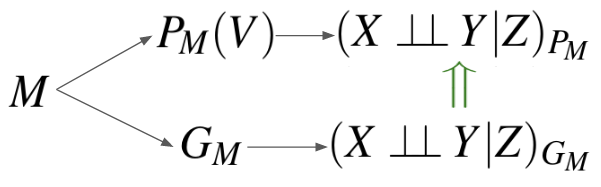
\includegraphics[width=.35\linewidth]{pics/my_own/dsep_Markov_flow.png}
\caption{When $M$ is solvable, the green implication is the directed global Markov property (validity of $d$-separation).}
\label{fig:dsep-Markov-flow}
\end{figure}

\subsection{Literature Review and Framework Selection}

The attractiveness of incorperating feedback into causality has already attracted significant intellectual effort, although a clear consensous has not yet been reached regarding what mathematical formulation to use. Perhaps the most intuitive approach to those familiar with DAG-based causality, is to unravel the feedback by duplicating the endogenous variables and indexing w.r.t time. However, as \cite{LearningLinear} points out, this model breaks down if the rate at which data is sampled is significantly slower than the feedback frequency. 

Settable systems are a well-known framework for cyclic causality \cite{White&Chalak} which I considered using, as it has proven insightful for game theory \cite{GameIncomplete}. The primary strength of settable systems lies in its convenient treatment of multiple equilibria. However, since stable-Lipschitz SCMs do not have multiple equilibria, this is more functionality than is needed right now. Settable systems also rely on fairly low-level representations of the optimization pressure on the equilibria (in order to select one equilibria from many) \cite{CausalGames}, and the addition of additional variables for distinguising between equilibria is more of a departure from \cite{pearl_2009} than is currently needed for this research.

Meanwhile, the modeling framework for \emph{cyclic SCMs} of \cite{Foundations} is, at least in spirit, very similar to Pearl's framework for acyclic SCMs \cite{pearl_2009}.
Cycles are incorporated simply by allowing the structural function $F$ of the SCM $M=(U,V,F,P(U))$ to be cyclic, that is, dependent on any variables in $U\cup V$.
This framework is currently developed for atomic interventions (which the authors rename `perfect interventions').
The authors take a more abstract approach than either of the two alternatives discussed above, for better and for worse. Consequently, this framework makes it straightforward to show the inheritance of properties between various classes of SCMs.

% There are several aspects of this framework which contrast with Pearl \cite{pearl_2009}.
% The authors emphasize almost-everywhere equivalence, with respect to the observational, interventional, and counterfactual distributions, or structural functions themselves. This emphasis implicitly impacts their definitions. For example, and notably, the definition of a variable's `parents' excludes any trivial dependencies. While this definition is semantically useful (we only say there's a parent if there's a dependence that really can't be ignored) it can be slightly confusing: for example, consider the two-node linear system of $x_1 = f_1(x_1,x_2)=0.5x_1+0.1x_2$ and $x_2 = f_2(x_1,x_2)=0.1x_1+0.5x_2$. According to the definitions of \cite{Foundations}, $x_1$ and $x_2$ are both parents of each other, yet no self-cycles exist, because there exists an SCM which is asymptotically equivalent without self-cycles. (This property of linear systems is discussed further in \cite{LearningLinear}).

I have opted to use the framework of cyclic SCMs for now, because 1. the inheritance of properties makes proofs more clear, 2. it seems overall the most similar to Pearl's framework in \cite{pearl_2009}, and 3. it has also been shown applicable to modeling game theory \cite{CausalGames}.

\begin{figure}
\centering
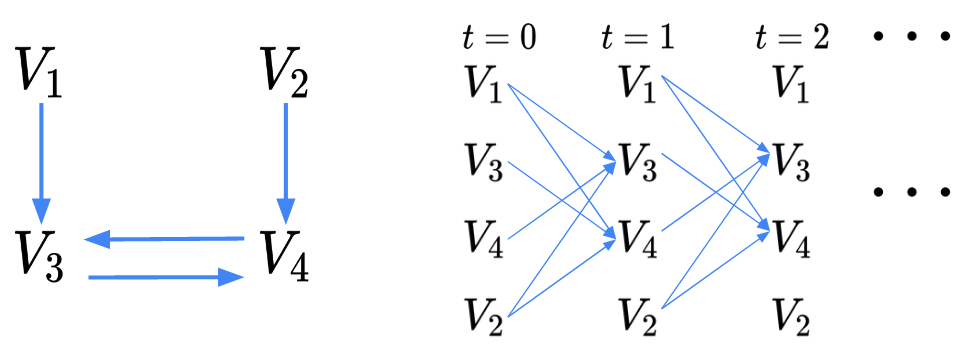
\includegraphics[width=.5\linewidth]{pics/my_own/rolled_out.png}
\caption{Left: The cyclic graph corresponding to the structural equations of Examples \ref{ex:cyclic-linear} and \ref{ex:cyclic-nonlinear}. Right: Rolling out this graph to explicitly represent the transient dynamics.}
\label{fig:rolled-out}
\end{figure}


\newpage
\subsection{Modeling Assumptions of Cyclic SCMs}\label{modeling}

The primary goal of cyclic SCMs is to remove the modeling assumption that causal relationships are all acyclic. While this is a huge step towards realistic modeling, the current formulation of cyclic SCMs in \cite{Foundations} still has several problematic assumptions.

The following two assumptions are necessary for cyclic SCMs to be an effective model of a phenomenon involving feedback:

\textbf{Assumption 1}: The sampling frequency is much lower than the feedback frequency.

\textbf{Assumption 2}: The noise frequency is much lower than the feedback frequency.

How realistic are these assumptions? Pepe agrees with me that Assumption 1 is valid for GDP measurements, because the accounting process significantly slows down measurement frequency. However, Assumption 1 is not valid for high-frequency trading (where we have extremely granular measurements).

Even more problematically, Assumption 2 explicitly contradicts the modeling assumptions economists often use for structural equation models:
\begin{itemize}
	\item Economists sample a new shock (aka. noise; exogenous variable) at each timestep.
	\item They either assume each timestep is a DAG, or use autogregressive relationships between each timestep and the next. 
\end{itemize}

In contrast, cyclic SCMs \cite{Foundations} sample a noise term at the start, and then use that fixed term throughout the evolution of all the dynamics! 
So, while cyclic SCMs remove one huge modeling assumption for practical economics (the structural equations are recursive), they still hold onto another huge assumption: shocks occur infrequently. 

Weakening these two assumptions is currently outside the scope of this report. However, I conjecture that Assumption 2 can be weakened for simple-Lipschitz SCMs (as is discussed further in Section \ref{noise}).

\subsection{Previous Results regarding D-separation}

\begin{figure}
\centering
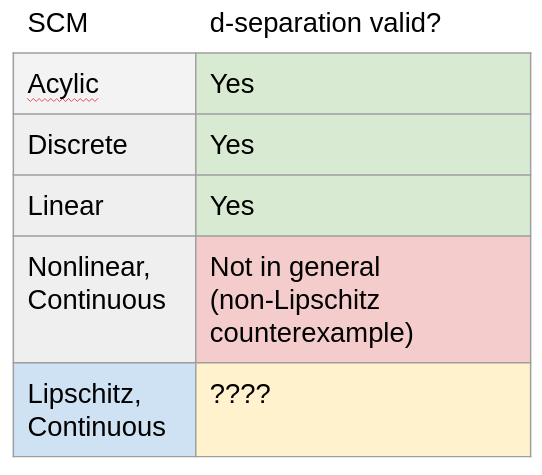
\includegraphics[width=.4\linewidth]{pics/my_own/review.png}
\caption{Classes of SCMs known to satisfy the directed global Markov property, as summarized by \cite{Foundations}. Here \emph{discrete} and \emph{continuous} refer to the domains of the exogenous and endogenous variables.}
\label{fig:review}
\end{figure}

\begin{figure}
\centering
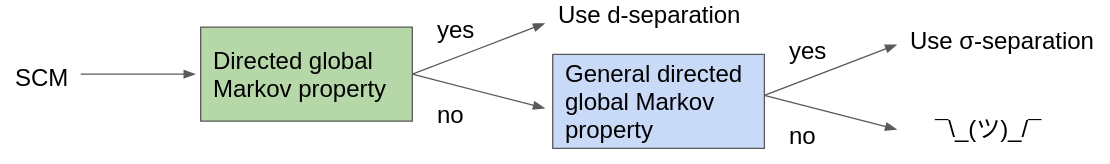
\includegraphics[width=.8\linewidth]{pics/my_own/inputs_outputs.png}
\caption{Relationship between $d$-separation and $\sigma$-separation.}
\label{fig:inputs-outputs}
\end{figure}

Acyclic SCMs, discrete SCMs (with ancestrally unique solvability), and linear SCMs (with nontrivial dependencies and positive measure) are known to satisfy the directed global Markov property \cite{MarkovCyclesLatent}. On the other hand, simple SCMs are known to satisfy the general directed global Markov property \cite{Foundations}. These results are summarized in Figure \ref{fig:review}.

When $d$-separation is not valid (the directed global Markov property does not hold), it may be that a weaker condition is satisfied. $\sigma$-separation is an extension of $d$-separation, which works by applying $d$-separation to the acyclification of the original graph. $\sigma$-separation implies $d$-separation; in other words, the general directed global Markov property is weaker than the directed global Markov property. The relationship between these two Markov properties can be seen in Figure \ref{fig:inputs-outputs}.

\emph{Simple SCMs} (presented in \cite{Foundations}) satisfy $\sigma$-separation but not $d$-separation. Simple SCMs are defined as SCMs which are uniquely solvable with respect to every subset of variables. Consequently, they preserve many of the properties of acyclic SCMs: the observational, interventional, and counterfactual distributions exist and are unique. Furthermore simple SCMs are closed under marginalization, and the causal semantics of the causal diagram's subgraph match the structure of the submodel of the SCM.

% \newpage
\subsection{Summary of Main Results}

The primary contributions of this paper are as follows, with the shorthand of dGMP := Directed Global Markov Property (a.k.a. “Validity of d-separation”).

\begin{itemize}
  \item Theorems
  \begin{itemize}
    \item acyclic SCMs $\subset$ stable-Lipschitz SCMs $\subset$ simple SCMs
    \item stable-Lipschitz SCMs are closed under interventions
    \item \textbf{Obs. D-separation}: The observational distribution of stable-Lipschitz SCMs satisfies dGMP
    \item Validity of Backdoor Criterion on stable-Lipschitz SCMs
    \item \textbf{Int. D-separation}: The interventional distribution of stable-Lipschitz SCMs satisfies dGMP
    \item stable-Lipschitz SCMs are closed under twin-operation

  \end{itemize}
  \item Numerics
  \begin{itemize}
    \item Obs. D-separation (above)
    \item The observational distribution of (non-stable) Lipschitz SCMs also satisfy dGMP
  \end{itemize}
\end{itemize}

\subsection{Paper Organization}
This paper is organized as follows. 
First, Section \ref{intuition} discusses the intution of the relationship between dynamics and potential response functions, by exploring three examples of increasing complexity.
Next in Section \ref{cyclic-d-sep}, we examine a case study for how d-separation can fail, from several perspectives, and how it can be modified to be stable-Lipschitz. 
That this example satisfies d-separation sets up the main theorems of Section \ref{main}.
Numerical investigations of these results are presented in Section \ref{numerics}. The relevance for economics in particular is discussed in Section \ref{real}.
Section \ref{future} discusses the next steps of the research.


\section{Dynamics and Potential Responses}\label{intuition}

Let’s examine how the dynamics and potential response functions change as we increase the complexity of the SCM, while introducing some important definitions along the way:
\begin{itemize}
  \item acyclic, linear SCMs (Example \ref{ex:acyclic-linear})
  \item cyclic, linear SCMs (Example \ref{ex:cyclic-linear})
  \item cyclic, nonlinear SCMs (Example \ref{ex:cyclic-nonlinear})
\end{itemize}

\subsection{Acyclic, Linear}

Acyclic SCMs have the property that once the values of early nodes are fixed, later nodes in the topological ordering are uniquely determined. For causal models with feedback to have this same behavior, there must exist unique solutions to subsets of the structural equations.

\begin{definition}[Unique Solvability]
Let $M=\langle V,U,F,P(U)\rangle$ be an SCM and $\mathbf{Z}\subseteq\mathbf{V}$ a subset of endogenous variables. We say that $M$ is uniquely solvable w.r.t. $\mathbf{Z}$ if for almost every $\mathbf{u}\in\text{dom}(\mathbf{U})$ and $\mathbf{v}_{\setminus\mathbf{Z}}\in\text{dom}(\mathbf{V}_{\setminus\mathbf{Z}})$ the equations
\[
\mathbf{V}_{\mathbf{Z}} = F_{\mathbf{Z}}(\mathbf{V},\mathbf{u})
\]
have a unique solution. If $\mathbf{Z}=\mathbf{V}$, we say that M is uniquely solvable.
\end{definition}

(\cite{Foundations} proves the equivalence of this condition with that of `mapping fixed inputs to unique outputs', which will be made clear with Example \ref{ex:acyclic-linear}).

Throughout this paper we only consider uniquely solvable SCMs, so we may use the following defintion of \emph{potential response}.

\begin{definition}[Potential Response]\label{defn:potential-response}
Let $M=\langle V,U,F,P(U)\rangle$ be a uniquely solvable SCM. 
The potential response function is the mapping $\overline{\mathbf{V}}(\mathbf{U}):\text{dom}(\mathbf{U})\to\text{dom}(\mathbf{V})$ which associates each $\mathbf{u}\in\text{dom}(\mathbf{U}$) with the unique solution $\mathbf{v}^*$ of $\mathbf{V} = F(\mathbf{V},\mathbf{u})$.
\end{definition}

The following example solidifies these concepts.

\begin{example}[Acyclic, Linear SCM]\label{ex:acyclic-linear}
Consider the following acyclic, linear SCM
\[
M_1 = 
\begin{cases}
\mathbf{u}, \mathbf{v}\in \mathbb{R}^4, \quad U_i \sim \mathcal{N}(0,1) \quad iid. \\
f_1:V_1\leftarrow U_1 \\
f_2:V_2\leftarrow U_2 \\
f_3:V_3\leftarrow \frac{2}{3}V_1+\frac{1}{3}V_2+\frac{4}{3}U_3+\frac{2}{3}U_4 \\
f_4:V_4\leftarrow \frac{1}{3}V_1+\frac{2}{3}V_2+\frac{2}{3}U_3+\frac{4}{3}U_4
\end{cases}
\]
where $\mathcal{N}(0,1)$ is Gaussian.
The causal graph of $M_1$ is shown in Figure \ref{fig:acyclic-graph}.

To evaluate the potential response $\overline{\mathbf{V}}(\mathbf{U})$ of $M_1$, we may sample $\mathbf{u}\in\mathbf{U}$ and consider the limit
\[
\overline{\mathbf{V}}(\mathbf{U})= \lim_{k\to\infty}F_{\mathbf{U}=\mathbf{u}}^{(k)}(\mathbf{V}_0)
\]
In this example, the limit exists and is unique because $M_1$ is acyclic. In fact, the dynamics converge within a single timestep, as shown (for the particular $\mathbf{u}=(-7,-2,2.5,7.5)$) in Figure \ref{fig:dynamics} (left).

In this case we can evaluate the potential response analytically for any $\mathbf{u}\in\mathbf{U}$ as
\begin{align*}
\overline{V_1}(\mathbf{U}) &= U_1 \\
\overline{V_2}(\mathbf{U}) &= U_2 \\
\overline{V_3}(\mathbf{U}) &= \frac{2}{3}U_1+\frac{1}{3}U_2+\frac{4}{3}U_3+\frac{2}{3}U_4 \\
\overline{V_4}(\mathbf{U}) &= \frac{1}{3}U_1+\frac{2}{3}U_2+\frac{2}{3}U_3+\frac{4}{3}U_4
\end{align*}
\end{example}

Example \ref{ex:acyclic-linear} highlights why unique solvability is such a desirable property of cyclic SCMs: the choice of the initialization $\mathbf{v}_0$ is `washed-out'. In general, cyclic SCMs may not be solvable at all, or the equilibria may not be unique; furthermore, these properties are not generally invariant under interventions or marginalizations \cite{Foundations}.

\begin{figure}
\centering
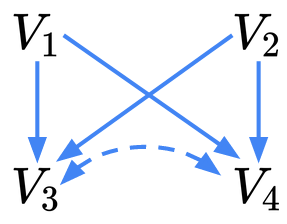
\includegraphics[width=.2\linewidth]{pics/my_own/acyclic_graph.png}
\caption{The causal graph of Example \ref{ex:acyclic-linear}.}
\label{fig:acyclic-graph}
\end{figure}

\begin{figure}
\centering
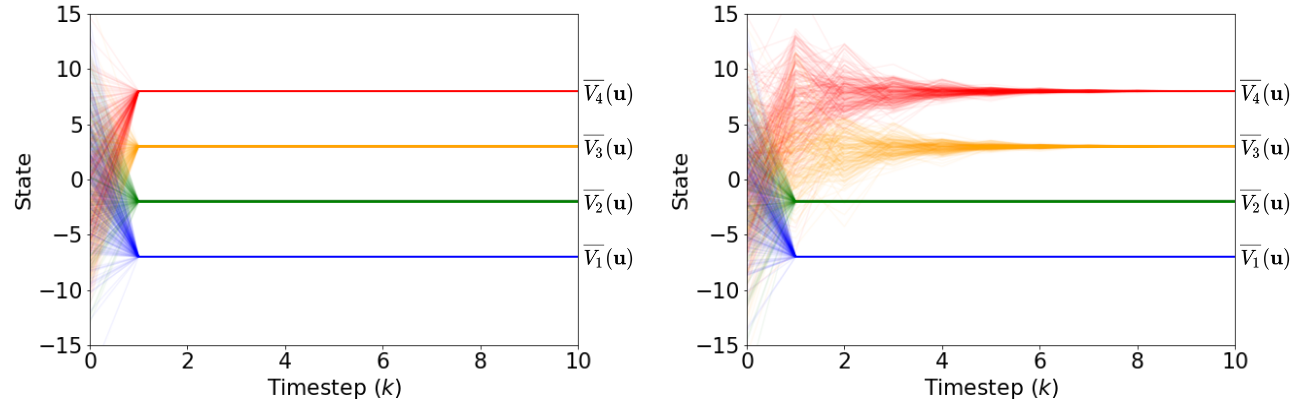
\includegraphics[width=\linewidth]{pics/my_own/example_dynamics.png}
\caption{The dynamics of Example \ref{ex:acyclic-linear} (left) and Example \ref{ex:cyclic-linear} (right), with fixed $\mathbf{u}=(-7,-2,2.5,7.5)$, and initialization $\mathbf{v}_0\sim\mathcal{N}(0,5)$.}
\label{fig:dynamics}
\end{figure}

\subsection{Cyclic, Linear}

Now, let us consider a cyclic, linear SCM, which is otherwise as close to Example \ref{ex:acyclic-linear} as possible.

\begin{example}[Cyclic, Linear SCM]\label{ex:cyclic-linear}
Consider
\[
M_2 = 
\begin{cases}
\mathbf{u}, \mathbf{v}\in \mathbb{R}^4, \quad U_i \sim \mathcal{N}(0,1) \quad iid. \\
f_1:V_1\leftarrow U_1 \\
f_2:V_2\leftarrow U_2 \\
f_3:V_3\leftarrow \frac{1}{2}V_1+\frac{1}{2}V_4+U_3 \\
f_4:V_4\leftarrow \frac{1}{2}V_2+\frac{1}{2}V_3+U_4
\end{cases}
\]
The causal graph of $M_2$ is shown in Figure \ref{fig:rolled-out} (left).
Note that there are now two edges between $V_3$ and $V_4$, as each depends on the other.

As Figure \ref{fig:dynamics} (right) shows, the feedback of the structural equations delays convergence of the endogenous variables to the fixed point. Note however, that nodes $V_1$ and $V_2$ precede the strongly connected component $\{V_3,V_4\}$ in the topological ordering, and converge immediately (as if they were acyclic).

By construction, $M_1$ and $M_2$ have the same potential response $\overline{\mathbf{V}}(\mathbf{U})$:
\begin{align*}
\overline{V_1}(\mathbf{U}) &= U_1 \\
\overline{V_2}(\mathbf{U}) &= U_2 \\
\overline{V_3}(\mathbf{U}) &= \frac{2}{3}U_1+\frac{1}{3}U_2+\frac{4}{3}U_3+\frac{2}{3}U_4 \\
\overline{V_4}(\mathbf{U}) &= \frac{1}{3}U_1+\frac{2}{3}U_2+\frac{2}{3}U_3+\frac{4}{3}U_4
\end{align*}
Thus, $M_1$ and $M_2$ are observationally equivalent; that is, they induce the same observational distribution, even though one has feedback and the other does not. Note that in this case, modeling the feedback in $M_2$ produces a simpler structural form than $M_1$.
\end{example}

In general, if a cyclic SCM is linear, so is its potential response (if it exists). To see this, note that for linear structural equations $F(\mathbf{V}) = B\mathbf{V}+\mathbf{U}$ we can derive the general form of the potential response as $\overline{\mathbf{V}}=(I-B)^{-1}\mathbf{U}$ whenever $\text{det}(I-B)\neq 0$.

For linear (cyclic) SCMs, the Lipschitz bound on the dynamics is particularly easy to evaluate, as it amounts to taking the entry-wise absolute-value of the transition matrix: $\lvert A\rvert$. More generally, we use the following defintion adopted from \cite{ReberIntrinsic}:

\begin{definition}[Lipschitz Matrix]\label{defn:lipschitz}
Let $M=\langle V,U,F,P(U)\rangle$ be an SCM, with $\text{dom}(\mathbf{U})=\R^m$, $\text{dom}(\mathbf{V})=\R^n$, and $F:\text{dom}(\mathbf{U})\times \text{dom}(\mathbf{V})\to\text{dom}(\mathbf{V})$ differentiable and Lipschitz.

Let $\mathbf{Z}\subseteq\mathbf{V}$ be a subset of endogenous variables.
For each pair of vertex indices $i$, $j\in\mathbf{Z}$, define
\[
a_{ij} = \sup_{\mathbf{u},\mathbf{v}} \left\lvert\frac{\partial f_i}{\partial v_j}(\mathbf{u},\mathbf{v})\right\rvert
\]
We call the matrix $A_{\mathbf{z}}=[a_{ij}]_{i,j\in\mathbf{Z}}$ the Lipschitz matrix of $F_\mathbf{Z}$.

When $\mathbf{Z}=\mathbf{V}$, we simply call $A=[a_{ij}]$ the Lipschitz matrix of $F$.
\end{definition}

Consider again Example \ref{ex:cyclic-linear}. The Lipschitz matrix of $M_2$ is 
\[
A =
\begin{bmatrix}
0 & 0 & 0 & 0 \\
0 & 0 & 0 & 0 \\
\frac{1}{2} & 0 & 0 & \frac{1}{2} \\
0 & \frac{1}{2} & \frac{1}{2} & 0 \\
\end{bmatrix}
\]
Note that $A$ is zero where there is no functional dependence, and otherwise represents the Lipschitz constant along the direction of each partial derivative.

The class of SCMs which are the focus of this paper are those whose strongly connected components have stable Lipschitz matricies (in order to ensure the unique solvability of the SCM).

\begin{definition}[stable-Lipschitz SCM]\label{stable-Lipschitz}
Let $M=\langle V,U,F,P(U)\rangle$ be an SCM with causal diagram $G$. 
We say $M$ is stable-Lipschitz if, for every strongly connected component $\mathbf{Z}$ of $G$, the following conditions hold:
\begin{itemize}
  \item $F_{\mathbf{Z}}$ is differentiable and Lipschitz.
  \item $\rho(A_\mathbf{Z})<1$.
\end{itemize}
where $\rho(A)$ is the spectral radius of $A$.
\end{definition}

Again returning to Example \ref{ex:cyclic-linear}, since the only strongly connected component in the causal graph (Figure \ref{fig:rolled-out}) is $\{V_3,V_4\}$, we construct the Lipschitz matrix
\[
A_{2,3} =
\begin{bmatrix}
\frac{1}{2} & \frac{1}{2} \\
\frac{1}{2} & \frac{1}{2} \\
\end{bmatrix}
\]
and check if the spectral radius of $A_{2,3}$ is less than $1$. In this case, $\rho(A_{2,3})=1$ so $M_2$ is \textbf{not} \emph{stable-Lipschitz}, even though it is \emph{stable} (always converges to the unique potential response found in Example \ref{ex:cyclic-linear}) and \emph{Lipschitz}.

\begin{remark}[Limitations of stable-Lipschitz]
As Example \ref{ex:cyclic-linear} highlights, the definition of simple-Lipschitz is quite restrictive (as is highlighted later by the numerics). However, this class has convienent theoretical properties which I expect to be valuable for proving Conjecture \ref{conj:stable-Lipschitz}.
\end{remark}



\subsection{Cyclic, Nonlinear}
Now we consider what the potential response function looks like, when the cyclic SCM in question is no longer linear (or even Lipschitz-continuous).

\begin{example}[Cyclic, Nonlinear SCM \cite{Acyclification}]\label{ex:cyclic-nonlinear}
Consider
\[
M_3 = 
\begin{cases}
\mathbf{u}, \mathbf{v}\in \mathbb{R}^4, \quad U_i \sim \mathcal{N}(0,1) \quad iid. \\
f_1:V_1\leftarrow U_1 \\
f_2:V_2\leftarrow U_2 \\
f_3:V_3\leftarrow V_1V_4+U_3 \\
f_4:V_4\leftarrow V_2V_3+U_4
\end{cases}
\]
$M_3$ respects the same causal graph as $M_2$, shown in Figure \ref{fig:rolled-out} (left).

The potential response $\overline{\mathbf{V}}(\mathbf{U})$ of $M_3$ can be solved for analytically as
\begin{align*}
\overline{V_1}(\mathbf{U}) &= U_1 \\
\overline{V_2}(\mathbf{U}) &= U_2 \\
\overline{V_3}(\mathbf{U}) &= \frac{U_1U_4 + U_3}{1-U_1U_2} \\
\overline{V_4}(\mathbf{U}) &= \frac{U_1U_4 + U_3}{1-U_1U_2}U_2 + U_4 \\
\end{align*}
In particular, note the singularity when $U_1U_2=1$. If $V_3$ and $V_4$ are observed to be large, then this means the exogenous variables are located near the singularity. This in turn implies that $V_1$ and $V_2$ are inversely proportional, so if $V_1$ is large, then $V_2$ is small. Consequently $(V_1 \nCI V_2 \mid V_3,V_4)_{P_{M_3}}$.

The Lipschitz matrix $A_{2,3}$ of the strongly connected component cannot be defined over this domain, since
\[
a_{31} = \sup_{\mathbf{v}\in\mathbf{V}}\lvert V_4\rvert \quad
a_{34} = \sup_{\mathbf{v}\in\mathbf{V}}\lvert V_1\rvert \quad
a_{42} = \sup_{\mathbf{v}\in\mathbf{V}}\lvert V_3\rvert \quad
a_{43} = \sup_{\mathbf{v}\in\mathbf{V}}\lvert V_2\rvert 
\]
are all unbounded over $\mathbf{u}\in \mathbb{R}^4$.
\end{example}

Thus, nonlinear cyclic SCMs can have singularities in their potential response functions, unlike linear SCMs. This consequently causes the Lipschitz matrix to be unbounded (and consequently not well-defined).


\begin{remark}
As discussed in \cite{Acyclification} (and further in \cite{Foundations}), Example \ref{ex:cyclic-nonlinear} is a counterexample to the claim that d-separation works in general for nonlinear, continous domained cyclic SCMs.
One way to see this (as pointed out by \cite{Acyclification}) is to solve for the induced observational distribution directly:

\[
P(\mathbf{V})=(\frac{1}{4\pi^2})e^{-\frac{v_1^2}{2}}e^{-\frac{v_2^2}{2}}e^{-\frac{(v_3-v_1v_4)^2}{2}}e^{-\frac{(v_4-v_2v_3)^2}{2}}\lvert(1-v_1v_2)^{-1}\rvert
\]
$P(\mathbf{V})$ cannot be factored completely into terms which not jointly contain $v_1$ and $v_2$
\end{remark}

\section{Cyclic D-separation}\label{cyclic-d-sep}

Surprisingly, even though we have $(V_1 \nCI V_2 \mid V_3,V_4)_{P_{M_3}}$ in the observational distribution of Example \ref{ex:cyclic-nonlinear}, we have $(V_1 \CI V_2 \mid V_3,V_4)_{G}$ according to d-separation. To evaluate the statement, we consider both paths from $V_1$ to $V_2$ as shown in Figure \ref{fig:paths}. Since each of these paths is blocked by $V_3$, $V_4$, we have that $(V_1 \CI V_2 \mid V_3,V_4)_{G}$.
Thus, d-separation fails to be valid in this example.

\begin{figure}
\centering
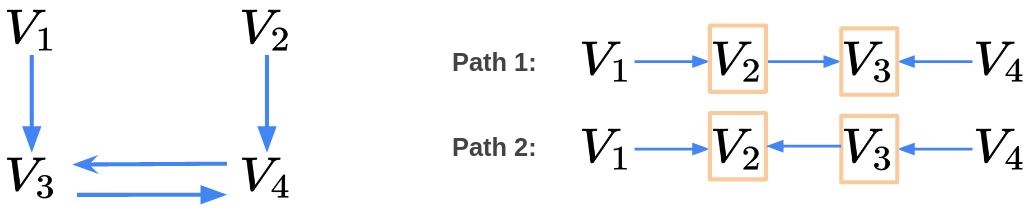
\includegraphics[width=0.7\linewidth]{pics/my_own/paths.png}
\caption{The paths which need to be considered to check $(V_1 \CI V_2 \mid V_3,V_4)_{G}$.}
\label{fig:paths}
\end{figure}


Even though $(V_1 \CI V_2 \mid V_3,V_4)_{G}$, $(V_1 \nCI V_2 \mid V_3,V_4)_{P_{M_3}}$ in Example \ref{ex:cyclic-nonlinear}, it seems that perhaps this failure of d-separation is due to the singluarity of the potential response function. 
In particular, note that the structural functions of Example \ref{ex:cyclic-nonlinear} are locally-linear. Perhaps if we restrict the domain of $M_3$ to where it behaves like a linear SCM, it will still preserve d-separation?

\begin{example}[Localization of an SCM]\label{ex:local}
Consider
\[
M_4 = 
\begin{cases}
\color{red}\mathbf{u}, \mathbf{v}\in [-0.5,0.5], \quad U_i \sim \mathcal{N}(0,1)\cap [-0.5,0.5] \quad iid. \color{black}\\
f_1:V_1\leftarrow U_1 \\
f_2:V_2\leftarrow U_2 \\
f_3:V_3\leftarrow V_1V_4+U_3 \\
f_4:V_4\leftarrow V_2V_3+U_4
\end{cases}
\]
the only difference from $M_3$ being that we restrict the domain of the exogenous variables (and hence, the endogenous variables) to be closer to $0$. 

Since the structural functions did not change, the potential response function is the same. However, the Lipschitz matrix $A_{2,3}$ is now well defined
\[
a_{31} = \sup_{\mathbf{v}\in\mathbf{V}}\lvert V_4\rvert = 0.5, \quad
a_{34} = \sup_{\mathbf{v}\in\mathbf{V}}\lvert V_1\rvert = 0.5,  \quad
a_{42} = \sup_{\mathbf{v}\in\mathbf{V}}\lvert V_3\rvert = 0.5,  \quad
a_{43} = \sup_{\mathbf{v}\in\mathbf{V}}\lvert V_2\rvert = 0.5 
\]
and satifies $\rho(A_{2,3})<1$. Hence, $M_4$ is stable-Lipschitz.
\end{example}

Indeed, by bounding the domain of $M_4$ away from the sigularity, then d-separation works, as Figure \ref{fig:counterexample_domain_restriction} demonstrates numerically, as we would expect if Problem \ref{prob:obs} resolves in the affirmative.
In order to test the conditional independence numerically over a continuous domain, the python package \verb|fcit| \cite{fcit} was used. The resulting p-values are distributed roughly uniformly on $[0,1]$, consistent with an \verb|fcit| result of conditional independence.


\begin{figure}
\centering
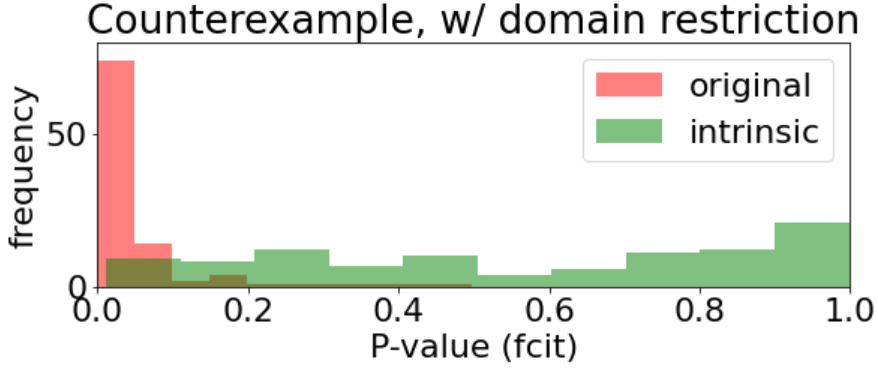
\includegraphics[width=.5\linewidth]{pics/my_own/counterexample_domain_restriction.png}
\caption{Numerical conditional tests of Examples \ref{ex:cyclic-nonlinear} and \ref{ex:local}. Here, conditional independence is tested while restricting the exogenous variables to be drawn from a truncated multivariate normal distribution (such that the SCM as a whole is intrinsically stable). The conditional independence identified by $d$-separation is now present in the observational distribution.}
\label{fig:counterexample_domain_restriction}
\end{figure}


\section{Main Results}\label{main}

Note that in Definition \ref{stable-Lipschitz} no constraints are placed on components of $F$ which \emph{are not} part of strongly connected components of $G$. This immediately implies the following reuslt:

\begin{theorem}[acylic $\subset$ stable-Lipschitz] \label{acyclic-subset}
Let $M$ be an acyclic SCM. Then $M$ is stable-Lipschitz.
\end{theorem}

Convienently, the restriction $\rho(A)<1$ in Definition \ref{stable-Lipschitz} is sufficient to ensure that stable-Lipschitz SCMs are uniquely solvable.

\begin{lemma}[Unique Solvability] \label{unique-solvable}
Let $M$ be a stable-Lipschitz SCM. Then $M$ is uniquely solvable.
\end{lemma}

\emph{Simple SCMs} are ones for which every submodel of the SCM is uniquely solvable. Recall from Definition \ref{defn:potential-response} that this is necessary for the existence of a unique potential response function:

\begin{definition}[Simple SCM \cite{Foundations}]
Let $M=\langle V,U,F,P(U)\rangle$ be an SCM. 
We call $M$ simple if $M$ is uniquely solvable w.r.t. every subset $\mathbf{Z}\subseteq\mathbf{V}$.
\end{definition}

Indeed, in \cite{Foundations} simple SCMs were proven to generalize a number of valuable properties about acyclic SCMs: 
\begin{itemize}
  \item the potential response function is always well-defined
  \item the observational, interventional, and counterfactual distributions always exist and are unique
  \item marginalizing over variables is always possible, and the causal semantics are always preserved
  \item $\sigma$ -separation always holds (the “general directed global Markov property”).
\end{itemize}

\emph{Stable-Lipschitz SCMs inherit all of these properties as well}, because they are in fact contained within the space of simple SCMs:

\begin{theorem}[stable-Lipschitz $\subset$ simple] \label{simple-subset}
Let $M$ be a stable-Lipschitz SCM. Then $M$ is simple.
\end{theorem}

Together, these two inclusions give us Figure \ref{fig:set-inclusion}.

In addition, stable-SCMs are closed under interventions:

\begin{theorem}[Closed under Interventions] \label{int-closed}
Let $M$ be a stable-Lipshitz SCM, $\mathbf{X}\subseteq\mathbf{V}$, and $\mathbf{x}\in\text{dom}(\mathbf{X})$. Then $M_{\text{do}(\mathbf{X}=\mathbf{x})}$ is stable-Lipschitz.
\end{theorem}
This fact is used for demonstrating that d-separation holds both for the observational, and the interventional distributions.



\begin{theorem}[Observational dGMP] \label{thrm:obs}
Let $M$ be stable Lipschitz with 1. structural equations of the form $F(\mathbf{V},\mathbf{U})=H(\mathbf{V})+\mathbf{U}$ (additive noise), 2. each $U_i\cap U_j=\emptyset$ for $i\neq j$ (independent noise), and 3. $P_M(\mathbf{V})$ has density according the the Legesgue measure on $\R^{|\mathbf{V}|}$ (positivity). 

Then $M$ satisfies the directed global Markov property.
\end{theorem}

I am confident that conditions 1 and 2 in the hypothesis can be substantially weakened with further research.

This is a very new result, so while I believe the proof to be accurate and comprehensive, I'm still vetting it for errors: I'd place 5:1 odds against finding an irrecoverable error in the proof. 

\begin{corollary}[Adjustment Formula] \label{adjustment}
Let $M$ be as in Theorem \ref{thrm:obs} and $Q=P(y|do(x))$ a causal query. If the BDC is satisfied, then $Q$ can be found via backdoor adjustment.
\end{corollary}

One of the motivations for weakening the condition of independent noise in Theorem \ref{thrm:obs} is to be able to similarly prove that the front-door criteria is also valid.

\begin{theorem}[Interventional dGMP] \label{thrm:int}
Let $M$ be as in Theorem \ref{thrm:obs}. For any $\mathbf{X}\subseteq \mathbf{Z}$, $M_{\text{do}(\mathbf{X}=\mathbf{x})}$ satisfies the directed global Markov property.
\end{theorem}

Because of their relation to \emph{intrinsic dynamical systems}, stable-Lipschitz SCMs are closed under a number of structural transformations (see Appendix \ref{intrinsic-appendix} for more details). In particular, they are closed under the twin operation:

\begin{theorem}[Closure under Twin Operation] \label{twin}
Let $M$ be stable-Lipschitz. Then $M^{\text{twin}}$ is also stable-Lipschitz.
\end{theorem}

\begin{conjecture}[Counterfactual dGMP] \label{thrm:counter}
Let $M$ be stable-Lipschtiz. Then the counterfactual distributions of $M$ satisfy the directed global Markov property relative to the corresponding twin network.
\end{conjecture}

I believe Conjecture \ref{thrm:counter} holds if the condition of independent noise in Theorem \ref{thrm:obs} can weakened, as an immediate consequence of Theorems \ref{thrm:int} and \ref{twin}. However, I would place 2:1 odds that I'm missing some additional aspect of the proof.

\section{Numerical Experiments}\label{numerics}

The claim of this report is pretty bold: d-separation holds for not only linear SCMs, but a wide range of nonlinear SCMs as well: this is an extension to a qualitatively different class of mathematical systems, within which linear SCMs are a mere set of measure 0. 

Numerical empiricism (e.g. randomly searching for counterexamples to a conjecture) provide an alternate mode of verification from traditional proofs: if both are pursued honestly, I expect making mistakes in a proof to occur fairly independently from making mistakes in experimental design or coding. (They're not completely seperate: missing an edge case in a proof is probably correlated with sampling bias in numerics, for example. But changing the paradigm makes it more likely to catch the omission).


When I discovered a mistake in my attempt at proving Theorem \ref{thrm:obs}, I sought to verify my conjecture numerically first, to guide my next research steps.
Specifically, I wanted to test my belief that stable-Lipschitz SCMs satisfy d-separation, and that non-stable Lipschitz SCMs do not.
Formally, these are the following two conjectures:

\begin{conjecture}[stable-Lipschitz]\label{conj:stable-Lipschitz}
Every stable-Lipschitz SCM satisfies the dGMP; that is, the observational distribution respects every conditional independence in the causal graph.
\end{conjecture}

\begin{conjecture}[Lipschitz]\label{conj:Lipschitz}
Lipschitz SCMs don’t generally satisfy the dGMP.
\end{conjecture}

I designed the following experiment:
\begin{enumerate}
  \item Generate all cyclic graphs of 4 nodes (totalling 107 non-isomorphic graphs)
  \begin{itemize}
  	\item We want as many nodes as possible, not because larger numbers are simply cooler, but because of the reality that complex graph structures (a.k.a. potential counterexamples) are only manifest in higher dimensions (because every 3-node structure is contained in the 4-nodes). 4 is as high as my laptop could handle.
  	\item 107 is an important number not because it is large, but because it is comprehensive. I mean to capture all graph structures: otherwise my sampling may happen to avoid inconvienent edge-cases. If someone replicating this experiment found there were in fact 109 non-isomorphic structures, that would indicate a serious flaw in my experimental implementation.
  \end{itemize}
  \item Given a graph, sample a neural network with Relu activations which respects that graph (and which has a spectral radius appropriate to the class of SCMs being tested)
  \begin{itemize}
  	\item Relu NNs were chosen for two reasons: 1. in general relu NNs have the univeral approximation property (caveat: that's not for NNs constrained to have repeating layers, as we're considering here), and 2. The Lipschitz matrix $A$ (Definition \ref{defn:lipschitz}) of a relu NN is easy to compute.
  	\item $\rho(|A|)<1$ for stable-Lipschitz, $\rho(A)<1$ for Lipschitz SCMs which converge to their fixed point; $\rho(A)>1$ for Lipschitz SCMs which don't technically converge to their fixed point.
  \end{itemize}
  \item Enumerate all possible d-separations for this graph
  \item For each independence claimed by d-separation, sample a dataset from the observational distribution 10 times (by means of sampling from $P(U)$, then applying root-finding methods to avoid numerical instability)
  \begin{itemize}
  	\item each dataset has 2100 samples, which appears sufficient for \verb|fcit| to have numerical stability
  	\item we want multiple pvals (10 was as many as my laptop could handle) for each independence check so we can avoid surious dependance claims.
  \end{itemize}
  \item Test whether the claimed independence from d-separation holds in each observation distribution using \verb|fcit|
\end{enumerate}

The surprising results of the numerics are aggregated in Figure \ref{fig:aggregated-plot}. Conjecture \ref{conj:stable-Lipschitz} holds (and indeed, I was able to finally prove Theorem \ref{thrm:obs} last week).

Surprisingly, however, Conjecture \ref{conj:Lipschitz} appears to be refuted! That is, the implicit belief I held that stable-Lipschitz was necessary for d-separation, was exposed as incorrect. 

So, not only does d-separation hold for stable-Lipschitz SCMs, it appears to hold for general Lipschitz SCMs as well! It will be interesting to see if the proof can be extended to Lipschitz SCMs.

\begin{figure}
\centering
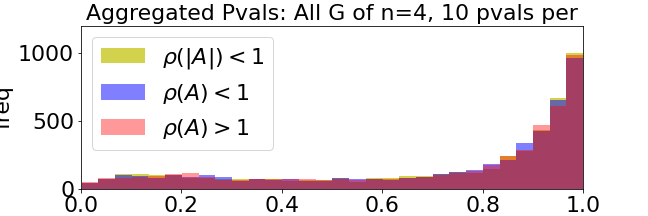
\includegraphics[width=.7\linewidth]{pics/my_own/aggregated_plot.png}
\caption{Aggregated pvals of conditional independence tests, across multiple SCMs. While each SCM was assessed individually, this plot clearly highlights the nigh-identical behavior of the three subclasses of Lipschitz SCMs that were tested. (I suspect the particular shape of the distribution may highlight something about fcit producing more confident independece predictions on certain graph structures (which were sampled equally among all three strata).)}
\label{fig:aggregated-plot}
\end{figure}


% \section{Research Report on Problem \ref{prob:obs}}\label{hole}

% \begin{figure}
% \centering
% 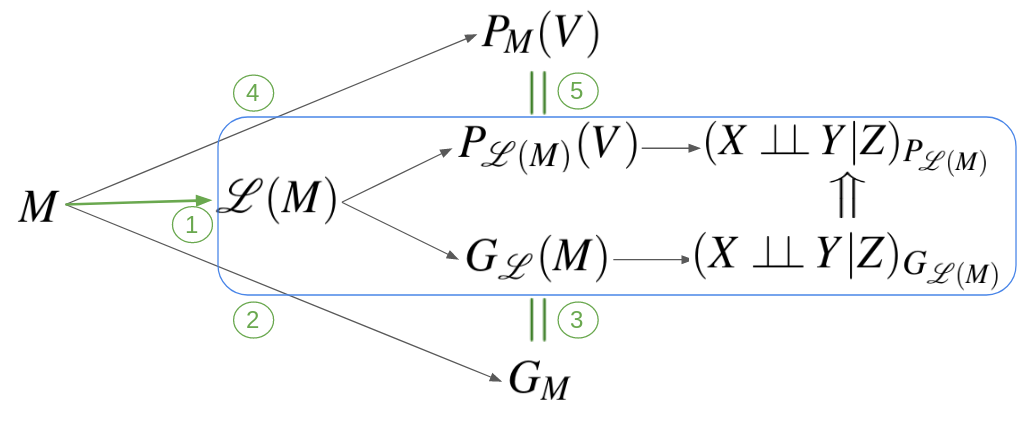
\includegraphics[width=.5\linewidth]{pics/my_own/research_plan_numbered_boxed.png}
% \caption{Incomplete proof sketch, for positive resolution of Problem \ref{prob:obs}. Note that the portion contained within the blue box simply expresses that the associated linear SCM $\mathcal{L}(M)$ satisfies the directed global Markov property (Figure \ref{fig:dsep-Markov-flow}).}
% \label{fig:research_plan_numbered_boxed}
% \end{figure}

% My research strategy for proving the affirmative of Problem \ref{prob:obs}, comprises of two parts (see Figure \ref{fig:research-plan-flow}): First, relate $M$ to a linear SCM $\mathcal{L}(M)$ which satisfies the directed global Markov property. Secondly, show that $M$ and $\mathcal{L}(M)$ respect the same graph and are observationally equivalent.

% This can be broken down into greater detail via Figure \ref{fig:research_plan_numbered_boxed}. Each of these lemmata (with a rough proof sketch) are described below:

% \begin{enumerate}
%   \item $M\rightarrow \mathcal{L}(M)$: Show that for every intrinsically-stable $M$, there exists a linear SCM $\mathcal{L}(M)$ which satisfies the directed global Markov property (the blue box).
%   \item $M\rightarrow G_M$: Always possible by definition, I believe.
%   \item $G_M = G_{\mathcal{L}(M)}$: Show that for every node, the parents are preserved (according to \cite{Foundations}'s definition of parents: see Appendix \ref{foundations-material}).
%   \item $M \rightarrow P_M(V)$: Show that if $M$ is intrinsically stable, it is uniquely solvable.
%   \item $P_M(V) = P_{\mathcal{L}(M)}(V)$: Translate intrinsic-stability property of $M$ and $\mathcal{L}(M)$ have the same equilibrium solutions, to SCMs. Show that this means they induce the same observational distributions.
% \end{enumerate}

\section{Application: Backdoor Adjustment and Macro Economics}\label{real}

Consider the following augmented supply and demand example, based on the classic supply-demand example from \cite{Foundations}. 

Suppose we have a hypothetical market for a “basket of goods”, as in Figure \ref{fig:supply-demand} (left). 
Here, we have the usual supply $S$, demand $D$ and price $P$ of this basket of goods; note that $P$ serves as a measure of inflation.
($P$ has a self-loop because it is a deterministic function of its previous value and $S$, $D$). Furthermore, we have an additional variable $X$ measuring the Federal Reserve interest rate. We assume that the interest rate affects demand $D$ significantly more than supply $S$ (for instance, if consumer credit availability is more immediately and significantly impacted than buisiness loan availability).

Suppose we have market + interest rate data from a period when the Federal Reserve is largely apolitical (so, basing decisions solely on inflation). 
What will the effect be of fixing the interest rate to a particular value regardless of inflation (say, due to politics)? (see Figure \ref{fig:supply-demand} (center))

\begin{figure}
\centering
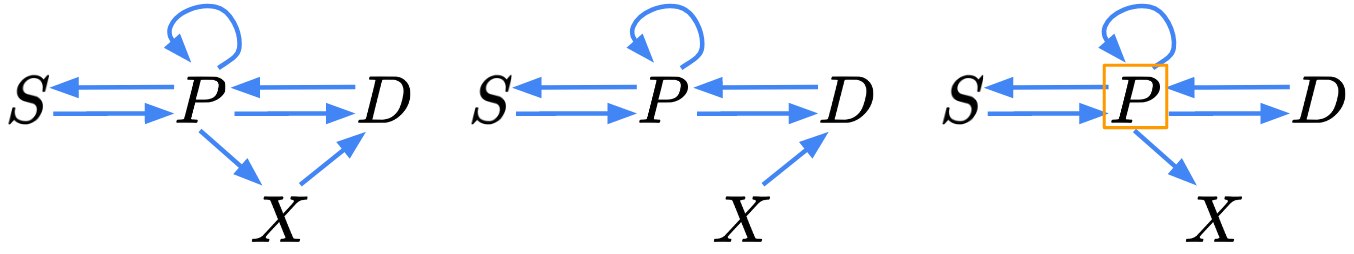
\includegraphics[width=\linewidth]{pics/my_own/supply_demand.png}
\caption{(left) A hypothetical market for supply/demand "basket of goods", with $P$ measuring inflation and $X$ the apolitical Federal Interest rate. (center) We would like to predict the effect of setting the interest rate to a fixed value, based on the observed apolitical data. (right) Since $(X \indep D | P)_{G_{\overline{X}}}$, we can perform backdoor adjustment.}
\label{fig:supply-demand}
\end{figure}

Since $(X \indep D | P)_{G_{\overline{X}}}$ (Figure \ref{fig:supply-demand} (right)), we can perform backdoor adjustment by Corollary \ref{adjustment} (assuming the underlying SCM is stable-Lipschitz and we have independent and additive $S$, $D$, and $X$ noise). Then, the effect of this new policy is identified from the previous data as
\[
P(D|do(x))=\sum_P P(D|x,p)P(p)
\]

\begin{remark}
We made a lot of assumptions along the way to that conclusion. Together with the problematic assumptions inherent to cyclic SCMs discussed in Section \ref{modeling}, I think this framework has a long way to go to being a competitive method of economic analysis. But as this example illustrates, it seems like that journey might be worth taking - the results would be rather tantalizing.
\end{remark}

\section{Future Work}\label{future}

This research only scratches the surface of an area previously seen as intractable. Consequently, I think there may be a lot of low-hanging fruit. 

\subsection{Pearl Causal Hierarchy}
\cite{Foundations} sets up a nice framework for the PCH, and suggest that the authors believe it holds, but stops short of actually making any claims about `collapse on a set of measure zero'.

To highlight why proving the PCH seems nontrivial to me, I invite you to imagine what a negative result might look like:
\begin{itemize}
  \item Even though the PCH holds for acyclic SCMs,
  \item since acyclic SCMs are themselves a set of measure 0 among the space of cyclic SCMs,
  \item it turns out that non-collapse is in fact the exception rather than the norm.
\end{itemize}

Nevertheless, I suspect the PCH will indeed hold for cyclic SCMs. But this should be demonstrated before spending lots of time on do-calculus or cyclic counterfactuals, for example, since if the PCH collapses then identification becomes much easier.

\subsection{Extending Observational dGMP}

As discussed following Theorem \ref{thrm:obs}, I believe the constraints of independent and additive noise can be weakened. Furthermore, the numerics suggest that even the assumption of simple-Lipschitz may be stronger than is necessary.

\subsection{Do-calculus}

The do-calculus would generalize the backdoor result of this report.

I suspect that the do-calculus should already follow from the current results of this report; however, I would like to take a fine-tooth comb through the validity proof of the acyclic do-calculus first, to ensure that everything generalizes properly to cyclic SCMs.

\subsection{Counterfactual dGMP}

Since the dGMP has been proven to hold for both the observational and interventional distributions of simple-Lipschitz SCMs, it is natural to ask if it also holds for counterfactual distributions:

\begin{problem}[stable-Lipschitz SCMs and $d$-separation: Counterfactual]
\label{prob:count}

Prove whether the counterfactual distribution of stable-Lipschitz SCMs satisfy the directed global Markov property: that is, whether every conditional independence read-off by $d$-separation in the twin network holds in the corresponding counterfactual distribution of the twin SCM.
\end{problem}

\subsection{Multiple Equilibria}

I conjecture that the results of this report may generalize nicely to non-uniquely-solvable SCMs, \emph{providing a general form of causal identification which does not care which equilibria is generating the potential response!}

This is the area of research I am most excited by, because currently the multiplicity of equlibria is a signicant difficulty for analysis of game theory and economics. Indeed, this is the fundamental premise of the settable systems framework \cite{White&Chalak}.

Settable systems takes an explicit approach toward modeling multiple equilibira. I conjecture that an implicit approach may be sufficient. In this way, a significant amount of additional modeling machinery of settable systems may be set aside.

My overall strategy for this direction basically consists of weakening the “uniquely solvable” condition to “solvable”, by showing that d-separation holds in the neighborhood of equilibria of “locally stable-Lipschitz” SCMs. 
Intuitively I think this should work because in some sense, knowing which equilibria we’re at is SCM-level knowledge – more than we should need for identification from the causal graph $G$ and $P(V)$.

\subsection{Noise Frequency}\label{noise}
As discussed in Section \ref{modeling}, cyclic SCMs make a problematic modeling assumption that noise (a.k.a. shocks in economics) occurs much less frequently than the feedback in the system; this is what allowed us to fix $\mathbf{u}\in\mathbf{U}$ and evaulate the potential response function.

I confidently conjecture that this assumption can be removed for stable-Lipschitz SCMs: that is, that for stable-Lipschitz SCMs we can allow a new $\mathbf{U}_t$ to be sampled at every timestep, and the induced behavior of the system will mimic the sequence of shocks (we will have independence to initial conditions $\mathbf{v}_0$; if the shocks stabilize, so will the dynamics). This result should follow directly from \cite{ReberIntrinsic, Switched}.

\section{Conclusion}
Despite being the natural modeling choice for phenomena involving feedback, cyclic causality has seen limited use because many of the convienent guarentees of acylic SCMs fail to hold for general cyclic SCMs. In particular, d-separation on the causal graph loses validity in the general cyclic setting!

In this report, we have presented research about the validity of d-separation (aka. the dGMP: directed global Markov property) for cyclic SCMs. Specifically, we proposed the class of stable-Lipschitz SCMs, which generalize acyclic SCMs and are contained by simple SCMs, thus inheriting all of the nice properties of simple SCMs. Stable-Lipschitz SCMs behave like linear SCMs asyptotically, and indeed, are proven to satsify the dGMP (currently with some additional assumptions).
These results are verified numerically, and the validity of the backdoor criterion is proven as well. We also show that stable-Lipschitz SCMs are closed under interventions, and that the interventional distributions of simple SCMs are similarly shown to satisfy the dGMP.

Lastly, we discussed further directions for research, including the Pearl Causal Hierarchy, the do-calculus, and most exciting, the possibility of causal identification with multiple equilibria.

\section{Acknowledgements}
This project is being submitted jointly for Elias Bareinboim's Causal Inference II course, and David Blei's Applied Causality course. I am indebted to both of their feedback and advice; as well as Alexis Bellot, my assigned mentor for CI2; and Pepe Montiel Olea, for discussing how to connect these results to economics.

% pdflatex main
% bibtex main
% pdflatex main
% pdflatex main

\bibliographystyle{plain}
\bibliography{refs}

\section{Appendix}

% \color{blue} Note: For epistemic transparency, I have highlighted claims in blue that I believe hold but need more rigor\color{black}. If I am not confident in a claim, I don't even mention it here (hence why Conjecture \ref{thrm:counter} is only a conjecture, even though I have almost all of it proved: there's still a significant hole that needs to be filled). I think this strikes the right balance, given that this report is meant to be a snapshot of my research progress, not a submission for peer-reviewed publication.

\subsection{Notation}
\begin{itemize}
  \item Lowercase letters (e.g. $z$) for particular values of random variables ($Z$); bold for sets of variables ($\mathbf{z}$ and $\mathbf{Z}$).
  \item $\text{dom}(X)$ denotes the domain over which the random variable $X$ is defined.
  \item $\sigma(A)$: The eigenvalues of a square matrix $A$.
  \item $\rho(A)$: the spectral radius of $A$.
  \item $An(\mathbf{Z})$: the ancestors of $\mathbf{Z}$ in a causal diagram, including $\mathbf{Z}$ itself.
  \item For matrices $A$ and $B$, $A \preceq B$ means that $a_{ij}\leq b_{ij}$ for all $i$, $j$.
\end{itemize}

\subsection{Proofs}

% \begin{theorem}[acylic $\subset$ stable-Lipschitz] \label{acyclic-subset}
% Let $M$ be an acyclic SCM. Then $M$ is stable-Lipschitz.
% \end{theorem}

\begin{proof}[Proof of Theorem \ref{acyclic-subset}: acylic $\subset$ stable-Lipschitz]
Let $G$ be the causal diagram of $M$. $G$ has no strongly connected components, so the conditions for stable-Lipschitz are vacuously satisfied.
\end{proof}

% \begin{theorem}[Closure under Interventions] \label{int-closed}
% Let $M$ be a stable-Lipshitz SCM, $\mathbf{X}\subseteq\mathbf{V}$, and $\mathbf{x}\in\text{dom}(\mathbf{X})$. Then $M_{\text{do}(\mathbf{X}=\mathbf{x})}$ is stable-Lipschitz.
% \end{theorem}

\begin{proof}[Proof of Theorem \ref{int-closed}: Closure under Interventions]
Let $G$ be the causal diagram of $M$. 

\underline{Case 1: $G$ is acyclic.}
Then $G_{\overline{\mathbf{X}}}$ is also acyclic, so vacuously $M_{\text{do}(\mathbf{X}=\mathbf{x})}$ is stable-Lipschitz.

\underline{Case 2: $G$ is strongly connected.}
Let $A$ be the Lipschitz matrix of $F$. Since $M$ is stable-Lipschitz, $\rho(A)<1$. Let $B$ be defined element-wise as 
\[
b_{ij} = 
\begin{cases}
  0 & i,j\in\mathbf{X} \\
  a_{ij} & \text{otherwise}
\end{cases}
\]
$B$ is the Lipschitz matrix for $M_{\text{do}(\mathbf{X}=\mathbf{x})}$, because $\text{do}(\mathbf{X}=\mathbf{x})$ sets each component function in $\mathbf{X}$ to a constant, inducing everywhere-zero partial derivatives. 
Furthermore, $0\preceq B \preceq A$, so $\rho(B)\leq\rho(A)<1$.
Thus, $M_{\text{do}(\mathbf{X}=\mathbf{x})}$ is stable-Lipschitz.

\underline{Case 3: $G$ contains multiple strongly connected components.}
Let $\{\mathbf{Z}_s\}$ be the set of the strongly connected components of $G$, and $\{\mathbf{W}_t\}$ the set of the set of the strongly connected components of $G_{\overline{\mathbf{X}}}$.
Since $G_{\overline{\mathbf{X}}}$ is a subgraph of $G$, we have that for each $\mathbf{W}_t$ there exists a $\mathbf{Z}_s$ such that $\mathbf{W}_t\subseteq\mathbf{Z}_s$.
Since $F_{\mathbf{Z}_s}$ is differentiable and Lipschitz by hypothesis, so is $F_{\mathbf{W}_t}$.
As in Case 2, let $A_{\mathbf{Z}_s}$ be the Lipschitz matrix of $F_{\mathbf{Z}_s}$, which by hypothesis satisfies $\rho(A_{\mathbf{Z}_s})<1$.
Let $B$ be defined over $\mathbf{Z}_s$ as
\[
b_{ij} = 
\begin{cases}
  a_{ij} & i,j\in\mathbf{W}_t \\
  0 & \text{otherwise}
\end{cases}
\]
Clearly $0\preceq B \preceq A_{\mathbf{Z}_s}$, so $\rho(B)\leq\rho(A_{\mathbf{Z}_s})<1$.
Since the principle submatrix $B_{\mathbf{W}_t}$ is precisely the Lipschitz matrix of $F_{{\mathbf{W}_t}}$, we have $\sigma(B_{\mathbf{W}_t})\subseteq \sigma(B)$. Thus $\rho(B_{\mathbf{W}_t})<1$.
Since $\mathbf{W}_t$ was an arbitrary strongly connected component, $M_{\text{do}(\mathbf{X}=\mathbf{x})}$ is stable-Lipschitz.
\end{proof}

% \begin{lemma}[Unique Solvability] \label{unique-solvable}
% Let $M$ be a stable-Lipschitz SCM. Then $M$ is uniquely solvable.
% \end{lemma}

\begin{proof}[Proof of Lemma \ref{unique-solvable}: Unique Solvability]
Let $G$ be the causal diagram of $M$. 

\underline{Case 1: $G$ is acyclic.}
It was proven in \cite{Foundations} that $M$ is uniquely solvable if it is acyclic.

\underline{Case 2: $G$ is strongly connected.}
Let $\mathbf{u}\in\text{dom}(\mathbf{U}$).
By \cite{ReberIntrinsic}, there exists a unique, globally attracting fixed point $\mathbf{v}^*\in\text{dom}(\mathbf{V})$ of the dynamical system $\big(F_{\mathbf{U}=\mathbf{u}}(\mathbf{V}),\mathbf{V}\big)$; that is, for all $\mathbf{v}_0\in\text{dom}(\mathbf{V})$, $\lim_{k\to\infty}F^{k}_{\mathbf{U}=\mathbf{u}}(\mathbf{v}_0)=\mathbf{v}^*$.
Thus the structural equations $\mathbf{V}=F(\mathbf{V},\mathbf{u})$ have the unque solution $\mathbf{v}^*$, so $M$ is uniquely solvable.

\underline{Case 3: $G$ is not strongly connected.}
Let $\{\mathbf{Z}_i\}_{i=1}^s$ be the set of strongly connected components of $G$ in topological order.
Let us partition the vertices not contained in strongly connected components, based on the order in which they impact a strongly connected component. Specifically, let $\{\mathbf{W}_i\}_{i=1}^{s+1}$ be defined as 
\begin{align*}
\mathbf{W}_1 &= An(\mathbf{Z}_1)\setminus \mathbf{Z}_1 \\
\mathbf{W}_2 &= An(\mathbf{Z}_2)\setminus (\mathbf{Z}_1\cup\mathbf{Z}_2\cup\mathbf{W}_1) \\
&\vdots \\
\mathbf{W}_s &= An(\mathbf{Z}_s)\setminus \big((\cup_{i=1}^s\mathbf{Z}_i)\cup(\cup_{i=1}^{s-1}\mathbf{W}_i))\big) \\
\mathbf{W}_{s+1} &= \mathbf{V}\setminus \big((\cup_{i=1}^s\mathbf{Z}_i)\cup(\cup_{i=1}^{s}\mathbf{W}_i))\big) \\
\end{align*}
where we may have a $\mathbf{W}_i=\emptyset$.
By construction, $\{\mathbf{Z}_i\}_{i=1}^s \cup \{\mathbf{W}_i\}_{i=1}^{s+1}$ forms a partition of $\mathbf{V}$, and $(\mathbf{W}_1,\mathbf{Z}_1,\hdots,\mathbf{W}_s,\mathbf{Z}_s,\mathbf{W}_{s+1})$ is a valid topological ordering of $G$.
Consequently, each $\{\mathbf{W}_1\}$, $\{\mathbf{W}_1,\mathbf{Z}_1\}$, $\{\mathbf{W}_1,\mathbf{Z}_1,\mathbf{W}_2\}$, etc. is ancestral in $G$.

We evaluate the solution of $\mathbf{V}=F(\mathbf{V},\mathbf{u})$ iteratively through $(\mathbf{W}_1,\mathbf{Z}_1,\hdots,\mathbf{W}_s,\mathbf{Z}_s,\mathbf{W}_{s+1})$ by pushing fixed values through each $\mathbf{W}_i$ to obtain a unique fixed output; evaluating each $\mathbf{Z}_i$ with these fixed inputs to obtain the unique fixed point of the dynamical system; feeding these newly fixed values through $\mathbf{W}_{i+1}$, and so on.
Specifically, because $\{\mathbf{W}_1\}$ is ancestral, we have $\mathbf{W}_1=F_{\mathbf{W}_1}(\mathbf{V},\mathbf{u})=F_{\mathbf{W}_1}(\mathbf{W}_1,\mathbf{u})$ which is acyclic, and so has a unique fixed point $\mathbf{w}_1^*$. Next, $\mathbf{Z}_1=F_{\mathbf{Z}_1}(\mathbf{V},\mathbf{u})=F_{\mathbf{Z}_1}(\mathbf{w}_1^*,\mathbf{Z}_1,\mathbf{u})$ has $\rho(A_{\mathbf{Z}_1})<1$, so by Case 2 produces a unique fixed point $\mathbf{z}_1^*$.
Next, $\mathbf{W}_2=F_{\mathbf{W}_2}(\mathbf{V},\mathbf{u})=F_{\mathbf{W}_2}(\mathbf{w}_1^*,\mathbf{z}_1^*,\mathbf{W}_2,\mathbf{u})$ is again acyclic, so produces a unique fixed point $\mathbf{w}_2^*$, and so on.

In this way we obtain a unique fixed point $\mathbf{v}^*$ for $\mathbf{V}=F(\mathbf{V},\mathbf{u})$ equal by stacking 
\[\mathbf{v}^*=[\mathbf{w}_1^*,\mathbf{z}_1^*,\hdots,\mathbf{w}_s^*,\mathbf{z}_s^*,\mathbf{w}_{s+1}^*]
\]
Thus $M$ is uniquely solvable.
\end{proof}


% \begin{theorem}[stable-Lipschitz $\subset$ simple] \label{simple-subset}
% Let $M$ be a stable-Lipschitz SCM. Then $M$ is simple.
% \end{theorem}

\begin{proof}[Proof of Theorem \ref{simple-subset}: stable-Lipschitz $\subset$ simple]
Let $\mathbf{u}\in\text{dom}(\mathbf{U})$, $\mathbf{Z}\subseteq\mathbf{V}$, and $\mathbf{w}\in\text{dom}(\mathbf{V}\setminus\mathbf{Z})$.
By Theorem \ref{int-closed}, $M_{\text{do}(\mathbf{w})}$ is stable-Lipschitz, and hence uniquely solvable by Lemma \ref{unique-solvable}.
This implies that there is a unique solution $\mathbf{v}^*$ to the equations $\mathbf{V}=F_{\text{do}(\mathbf{w})}(\mathbf{V},\mathbf{u})$.
By definition of $\text{do}(\mathbf{w})$ this is
\begin{align*}
\mathbf{Z} &= F_{\mathbf{Z}}(\mathbf{V},\mathbf{u}) = F_{\mathbf{Z}}(\mathbf{Z},\mathbf{W},\mathbf{u}) \\
\mathbf{W} &= F_{\mathbf{W}}(\mathbf{V},\mathbf{u}) = \mathbf{w} \\
\end{align*}
with the latter equation already solved.
Plugging this into the first equation, we obtain $\mathbf{Z} = F_{\mathbf{Z}}(\mathbf{Z},\mathbf{w},\mathbf{u})$, which must be uniquely solvable since we know $\mathbf{V}=F_{\text{do}(\mathbf{w})}(\mathbf{V},\mathbf{u})$ is uniquely solvable.

Since $\mathbf{u}\in\text{dom}(\mathbf{U})$ and $\mathbf{w}\in\text{dom}(\mathbf{V}\setminus\mathbf{Z})$ were arbitrary, we have that $M$ is uniquely solvable w.r.t. $\mathbf{Z}$.
Since $\mathbf{Z}\subseteq\mathbf{V}$ was arbitrary, $M$ is simple.
\end{proof}

\begin{lemma}[Injectivity] \label{injective}
Let $M$ have structural functions of the form $F(\mathbf{V},\mathbf{U})=H(\mathbf{V})+\mathbf{U}$ (additive noise). Furthermore, assume that for every ancestral $\mathbf{W}\subseteq \mathbf{V}$, 
\begin{itemize}
  \item $F_{\mathbf{W}}$ is Lipschitz
  \item $\text{det}(I_{|\mathbf{W}|}-A_\mathbf{W})\neq 0$ (uniquely solvable)
\end{itemize}
Then $h_\mathbf{V}:=\mathbf{V}-H(\text{Pa}(\mathbf{V}))$ is injective for ancestral $\mathbf{W}\subseteq\mathbf{V}$.
\end{lemma}

\begin{proof}
Assume $h_\mathbf{W}(\mathbf{w}^{(1)})=h_\mathbf{W}(\mathbf{w}^{(2)})$. This implies $\mathbf{w}^{(1)}-\mathbf{w}^{(2)} = K(\mathbf{w}^{(1)}) - K(\mathbf{w}^{(1)})$, so if we take the element-wise absolute value we have the element-wise inequality $\lvert\mathbf{w}^{(1)}-\mathbf{w}^{(2)}\rvert = \lvert K(\mathbf{w}^{(1)}) - K(\mathbf{w}^{(1)})\rvert\preceq A_\mathbf{W} \lvert\mathbf{w}^{(1)}-\mathbf{w}^{(2)}\rvert$. Thus $(I_{|\mathbf{W}|}-A_\mathbf{W})\lvert\mathbf{w}^{(1)}-\mathbf{w}^{(2)}\rvert\preceq 0$. By hypothesis $\text{det}(I_{|\mathbf{W}|}-A_\mathbf{W})\neq 0$ so $(I_{|\mathbf{W}|}-A_\mathbf{W})^{-1}$ exists, so in fact $\lvert\mathbf{w}^{(1)}-\mathbf{w}^{(2)}\rvert\preceq 0$. Thus $\mathbf{w}^{(1)}=\mathbf{w}^{(2)}$.
\end{proof}

% From Matrix Analysis, Theorem 8.1.18 of Edition 2
% \begin{lemma}[Intrinsic Stability] \label{intrinsic-stability}
% Let $A$ be a Lipschitz matrix for differentiable $H(\mathbf{V})$. Then $\rho(A)<1$ implies $\rho(\frac{dK}{d\mathbf{V}}(\mathbf{v}))<1$ for all $\mathbf{v}\in\mathbf{V}$.
% \end{lemma}

% \begin{proof}
% \color{blue} This was something Benjamin Webb and I used frequently. It holds numerically, I am confident it is true, yet I cannot find a proof to cite right now. I can prove it again though (or worst-case scenario, just make the hypothesis of the theorem slightly stronger.) \color{black}
% \end{proof}

% \begin{theorem}[Observational dGMP] \label{thrm:obs}
% Let $M$ be stable Lipschitz with 1. structural equations of the form $F(\mathbf{V},\mathbf{U})=H(\mathbf{V})+\mathbf{U}$ (additive noise), 2. each $U_i\cap U_j=\emptyset$ for $i\neq j$ (independent noise), and 3. $P_M(\mathbf{V})$ has density according the the Legesgue measure on $\R^{|\mathbf{V}|}$ (positivity). 

% Then $M$ satisfies the directed global Markov property.
% \end{theorem}

% \begin{remark}
% I am confident that conditions 1 and 2 in the hypothesis can be substantially weakened with further research.

% This is a very new result, so while I believe the proof to be accurate and comprehensive, I'm still vetting it for errors: I'd place 5:1 odds against finding an irrecoverable error in the proof. 
% \end{remark}

\begin{proof}[Proof of Theorem \ref{thrm:obs}: Observational dGMP]
We show that $M$ satisfies the SEPwared property of \cite{MarkovCyclesLatent} (Definition 3.8.14).
Let $h_\mathbf{V}:=\mathbf{V}-H(\text{Pa}(\mathbf{V}))$ leading to $h_\mathbf{W}(\mathbf{w})=\mathbf{U}_\mathbf{W}$ for ancestral $\mathbf{W} \subseteq \mathbf{V}$.
By Lemma \ref{injective}, $h_\mathbf{W}$ is bijective. 
Thus we can evaluate 
\[
\lvert h^\prime_{\mathbf{W}}(\mathbf{w})\rvert = \lvert \frac{dh_\mathbf{W}}{d\mathbf{w}}(\mathbf{w})\rvert=\lvert\text{det}(I_{|\mathbf{W}|}-\frac{dH_\mathbf{W}}{d\mathbf{w}}(\mathbf{w}))\rvert
\]
By similar reasoning to the proof of Theorem \ref{int-closed}, $\rho(A_{\mathbf{W}})<1$, and by definition $\lvert \frac{dH_\mathbf{W}}{d\mathbf{w}}(\mathbf{w}) \rvert \preceq A_{\mathbf{W}}$, so by Theorem 8.1.18 of \cite{MatrixAnalysis} we have that $\rho(\frac{dH_\mathbf{W}}{d\mathbf{w}}(\mathbf{w}))<1$ for all $\mathbf{v}\in\mathbf{V}$.
This constitutes a sufficient condition for 
\[
\lvert h^\prime_{\mathbf{W}}(\mathbf{w})\rvert =\lvert\text{det}(I_{|\mathbf{W}|}-\frac{dH_\mathbf{W}}{d\mathbf{w}}(\mathbf{w}))\rvert \neq 0 
\]
for all $\mathbf{v}\in\mathbf{V}$.
Thus, SEPwared holds, so by \cite{MarkovCyclesLatent} $M$ satisfies the dGMP.
\end{proof}

% \begin{corollary}[Adjustment Formula] \label{adjustment}
% Let $M$ be as in Theorem \ref{thrm:obs} and $Q=P(y|do(x))$ a causal query. If the BDC is satisfied, then $Q$ can be found via backdoor adjustment.
% \end{corollary}

\begin{proof}[Proof of Corollary \ref{adjustment}: Adjustment Formula]
The proof of the BDC relies on 1. a d-separation condition, 2. the directed global Markov property, and 3. axioms of probability. So long as we use cyclic d-separation, 1 can be checked. Theorem \ref{thrm:obs} provides 2, and 3 is unaffected.
\end{proof}

% \begin{remark}
% One of the motivations for weakening the condition of independent noise in Theorem \ref{thrm:obs} is to be able to similarly prove that the front-door criteria is also valid.
% \end{remark}

% \begin{theorem}[Interventional dGMP] \label{thrm:int}
% Let $M$ be as in Theorem \ref{thrm:obs}. For any $\mathbf{X}\subseteq \mathbf{Z}$, $M_{\text{do}(\mathbf{X}=\mathbf{x})}$ satisfies the directed global Markov property.
% \end{theorem}

\begin{proof}[Proof of Theorem \ref{thrm:int}: Interventional dGMP]
By Theorem \ref{simple-subset}, we have that $M$ is simple.
By \cite{Foundations}, this implies that $G_{\overline{\mathbf{X}}}=G_{M_{\text{do}(\mathbf{X}=\mathbf{x})}}$.
By Theorem \ref{int-closed}, we have that $M_{\text{do}(\mathbf{X}=\mathbf{x})}$ is also stable-Lipschitz.

All that remains is to show that the hypothesis of Theorem \ref{thrm:obs} still holds. Interventions do not change the structural form of $F$, so the additive noise condition still holds; similarly, independant noise is unaffected. Lastly, if $P_M(\mathbf{V})$ has density, so does $P_{M_{\text{do}(\mathbf{X}=\mathbf{x})}}(\mathbf{V})$.
Thus $M$ satisfies the dGMP.
\end{proof}

% \begin{theorem}[Closure under Twin Operation] \label{twin}
% Let $M$ be stable-Lipschitz. Then $M^{\text{twin}}$ is also stable-Lipschitz.
% \end{theorem}

\begin{proof}[Proof of Theorem \ref{twin}: Closure under Twin Operation]
By hypothesis, for each strongly connected component the corresponding $A_\mathbf{Z}$ satisfies $\rho(A_\mathbf{Z})<1$.
Note that the strongly connected components of $M^{\text{twin}}$ are as follows:
\[
\text{strong}(F^{\text{twin}})=\text{strong}(F)\cup\text{strong}(F^\prime)
\]
that is, simply duplicated.
Hence $A_\mathbf{Z}$ is the Lipschtiz matrix for both the original component and its duplicate, so indeed $M^{\text{twin}}$ is also stable-Lipschitz.
\end{proof}

% \begin{conjecture}[Counterfactual dGMP] \label{thrm:counter}
% Let $M$ be stable-Lipschtiz. Then the counterfactual distributions of $M$ satisfy the directed global Markov property relative to the corresponding twin network.
% \end{conjecture}

% \begin{remark}
% I believe Conjecture \ref{thrm:counter} holds if the condition of independent noise in Theorem \ref{thrm:obs} can weakened, as an immediate consequence of Theorems \ref{thrm:int} and \ref{twin}. However, I would place 2:1 odds that I'm missing some additional aspect of the proof.
% \end{remark}

\subsection{Intrinsic Dynamical Networks}\label{intrinsic-appendix}

Considered from a dynamical-systems perspective, intrinsically stable dynamical networks (the theoretical foundation for stable-Lipschitz SCMs) have a number of promising properties relevant to causality. They have a unique equilibrium, so the potential response function of the SCM will be well-defined. They `behave’ like linear systems: they are asymptotically bounded by the dynamics of a linear system, and share the same equilibria if subject to the same forcing factor (exogenous distribution). Intuitively speaking, this means that we can go to linear-world, prove things about the system there, and the results will still hold in nonlinear-world. Furthermore, intrinsically-stable systems are quite general: they only require Lipschitz-continuity, and the domain to be a product of metric spaces (which could be something nice like $\R^4$, or something abstract like language and shapes). If a general domain like metric spaces is used, the linearization uses the metrics to map to the real numbers: in this way the domain is simplified as well.

Of particular interest for causality, intrinsically-stable systems derive their name because they are closed under a surprising number of structural transformations; that is, the resulting system will still be intrinsically-stable, and often (if applicable) the equilibria will be preserved. Some especially relevant transformations are: lengthening of paths (i.e. through time-delays \cite{ReberIntrinsic}), collapsing portions of the graph \cite{IsospectralReduction}, duplicating portions of the graph (specialization \cite{Specialization}), time-varying structural switching \cite{Switched}, and any and all isospectral transformations (transformations which preserve the eigenvalues of the system \cite{IsospectralBook}).

\end{document}

%%% Local Variables:
%%% mode: latex
%%% TeX-master: t
%%% End:
